\chapter{Brain Viewer Tool}
\label{chap:brainviewer}
The final goal of explaining a model is to help a specialist to make a better diagnosis. Therefore it's important to provide him with a tool that is as easy as possible to use. For that we build a web app where a clinician can upload the brain he is interested in checking, and the attention map we computed in order to see them and navigate into them exactly the same way he already knows how to do using other visualization software such as SPM\footnotemark{}. In addition, he is also provided with information that tells him how confident the model is at predicting dementia and the ground truth label (see figure \ref{fig:brainViever_pred_output}). The control panel \ref{fig:brainViever_control_panel} enable a richer experience notably through raising the pixel intensity of the saliency map to the power of its slicer value. Therefore highlighting more the zone of the image where the model has more attention. Last but not least the checkbox allows the user to hide/display the brain or the saliency map for better visual control. An intuition of the capability of that tool can be sensed through the screenshot in figure \ref{fig:brain_viewer}. Or you could even try it live at \href{https://cgallay.github.com/MasterProject}{https://cgallay.github.com/MasterProject}.
\footnotetext{\href{https://www.fil.ion.ucl.ac.uk/spm/software/}{https://www.fil.ion.ucl.ac.uk/spm/software/}}

\begin{figure}
 \centering
 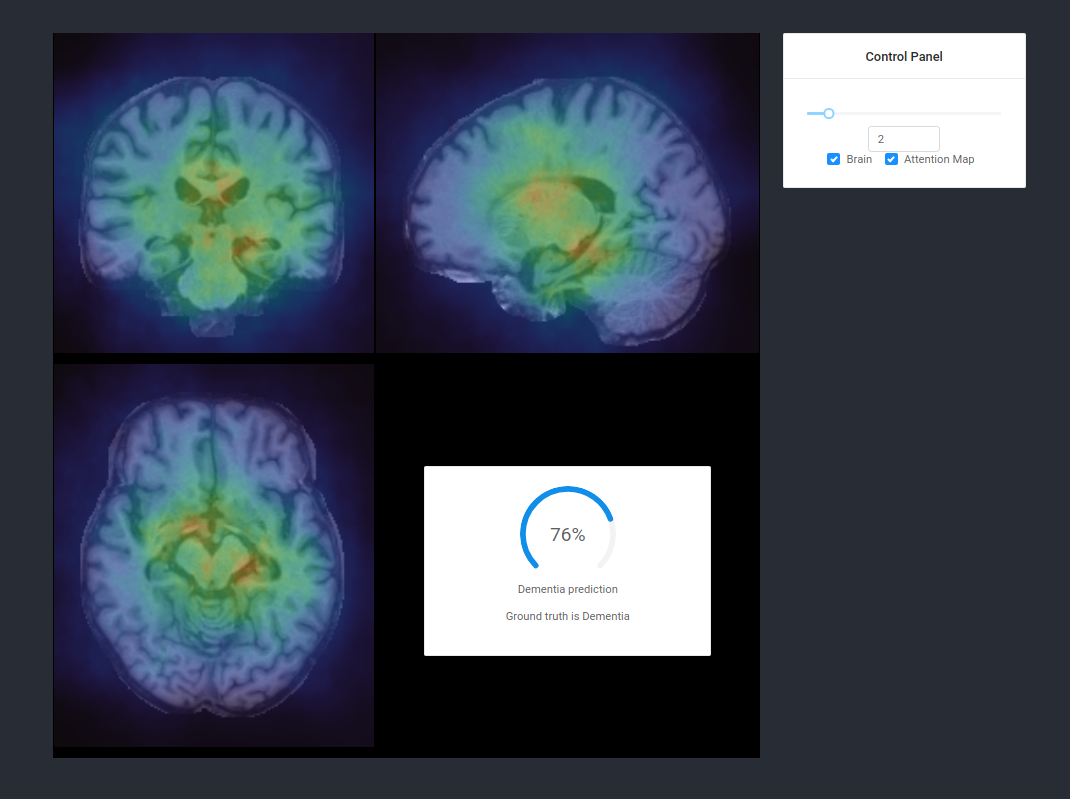
\includegraphics[width=.9\linewidth]{figures/BrainViewer/main.png}
 \captionsetup{width=.9\linewidth}
 \caption{Screenshot of the the viewer.}
 \label{fig:brain_viewer}
\end{figure}

\begin{figure}
\centering
\begin{subfigure}{.4\textwidth}
  \centering
  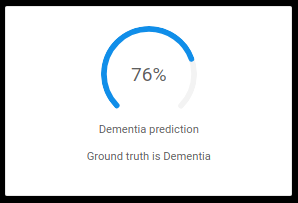
\includegraphics[width=1\linewidth]{figures/BrainViewer/info.png}
  \caption{Prediction output.}
  \label{fig:brainViever_pred_output}
\end{subfigure}%
\hfill
\begin{subfigure}{.4\textwidth}
  \centering
  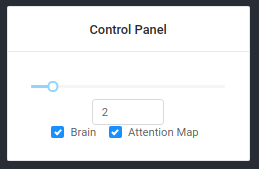
\includegraphics[width=1\linewidth]{figures/BrainViewer/control_panel.png}
  \caption{Control Panel.}
  \label{fig:brainViever_control_panel}
\end{subfigure}
\caption[Elastic]{Extra element of the BrainViewer tool.}
\label{fig:brainViwer_extra}
\end{figure}


\chapter{Age predictor}
\label{chap:age_pred}
\section{Training model}

\begin{wrapfigure}{r}{0.6\textwidth}
 \centering
 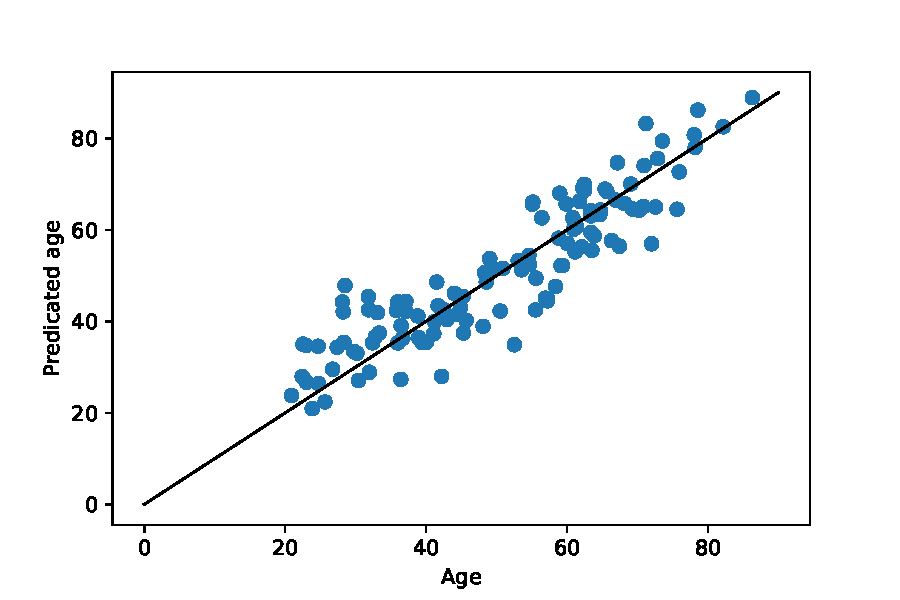
\includegraphics[width=.9\linewidth]{figures/Age_pred_vs_age_IXI.pdf}
 \captionsetup{width=.9\linewidth}
 \caption{Prediction of age versus real age on IXI test set.}
 \label{fig:IXI_pred_vs_age}
\end{wrapfigure}

At the very beginning of the project, we had no access to MRI from dement people. In order to proceed anyway and gain some time, we choose to work on predicting the age of someone based only on an MRI scan of his brain. For that purpose, the public IXI dataset was used. From there we design our preprocessing pipeline, and model that we were able to reuse later for dementia detection simply by changing the training dataset. We present here the result we obtained for that experience.

The only variation compared to the dementia detection pipeline explained earlier is the last layer of the model we used and the loss to optimized. Instead of a $Sigmoid$ function, the last layer for a regression simply does not contain any activation function. The loss we want to minimize is a mean square error, which is classic for regression as we want to penalize larger errors. To evaluate the performance, the Mean Absolute Error (MAE) was computed, as it is more meaningful and easier for a human to imagine.


We achieved an MSE of 45 which correspond to an MAE of roughly 5 years. Interestingly by looking at the correlation between our prediction error and the age of the patient in figure \ref{fig:IXI_pred_vs_age}, we found that the performance is uniform across ages which is a nice property of our predictor.

\section{Dementia seen as over ageing}
In this section, we tried to check whether or not a patient with dementia can be seen as an over aged person. By looking at figure \ref{fig:dem_vs_control_age_pred} it is hard to tell that indeed our age predictor trained on healthy brains is over ageing dement people. Indeed we might see that the model has worst performances on damage brain but once again we do not have enough data to conclude anything with certainty. 

Figure \ref{fig:dem_vs_control_age_pred} do indeed highlight age bias present in the dataset. 
\begin{figure}
 \centering
 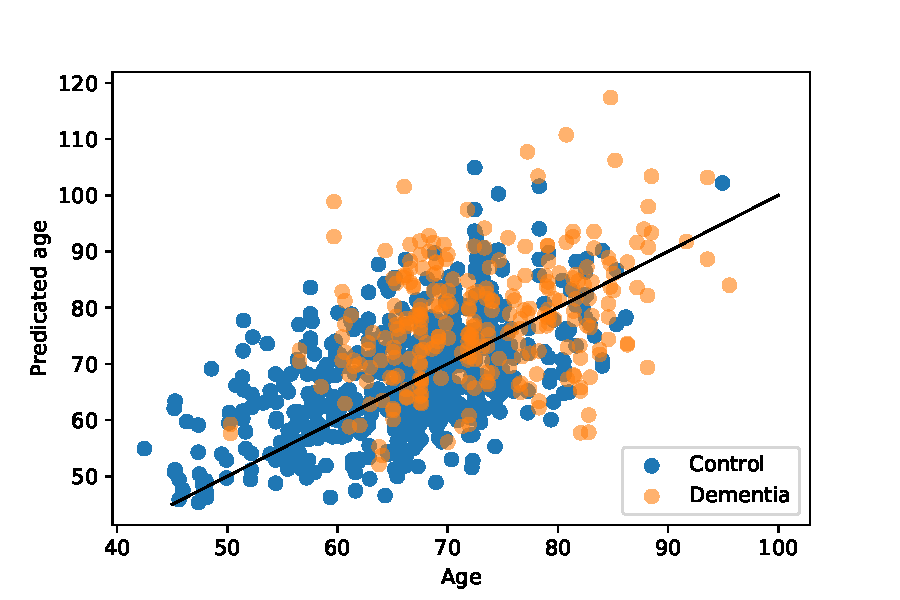
\includegraphics[width=.9\linewidth]{figures/Experiements/dem_vs_cont_age_pred.pdf}
 \captionsetup{width=.9\linewidth}
 \caption{Prediction of age for control and dement patient for OASIS dataset.}
 \label{fig:dem_vs_control_age_pred}
\end{figure}
